\documentclass[tikz,border=10pt]{standalone}
\usepackage{amsmath,amssymb}
\usepackage{tikz}
\usetikzlibrary{arrows,automata,backgrounds,calendar,chains,decorations,decorations.pathreplacing,decorations.text,fit,matrix,mindmap,patterns,petri,plotmarks,positioning,shadows,shapes,shapes.callouts,shapes.geometric,shapes.misc,spy,trees,calc,intersections,tikzmark,arrows.meta}
\usepackage{xcolor}
\usepackage{pgfplots}
\pgfplotsset{compat=1.16}

% Common math macros from the book
\def\x{\mathbf{x}}
\def\y{\mathbf{y}}
\def\z{\mathbf{z}}
\def\A{\mathbf{A}}
\def\b{\mathbf{b}}
\def\c{\mathbf{c}}
\def\w{\mathbf{w}}
\def\v{\mathbf{v}}
\def\u{\mathbf{u}}
\def\e{\mathbf{e}}
\def\zero{\mathbf{0}}
\def\R{\mathbb{R}}
\def\N{\mathbb{N}}
\def\Z{\mathbb{Z}}
\def\Q{\mathbb{Q}}
\def\st{\text{s.t.}}
\def\vect#1{\mathbf{#1}}
\def\xLP{x^{\mathrm{LP}}}
\def\zLP{z^{\mathrm{LP}}}
\def\xIP{x^{\mathrm{IP}}}

% Common node styles from the book
\tikzset{
    main/.style={circle, draw, fill=gray!20, minimum size=1cm, font=\normalsize},
    dot/.style={circle,fill=blue,minimum size=3pt,inner sep=0pt, outer sep=-1pt},
    vertex/.style={circle,fill=black!25,minimum size=20pt,inner sep=0pt},
    edge/.style={draw,-,thick},
    directed edge/.style={draw,->,>=latex,thick},
}

% Additional macros for 3D/coordinate systems
\newcommand{\xhat}{\hat{\x}}
\newcommand{\yhat}{\hat{\y}}
\newcommand{\zhat}{\hat{\z}}
\newcommand{\ihat}{\hat{\imath}}
\newcommand{\jhat}{\hat{\jmath}}
\newcommand{\khat}{\hat{k}}

\begin{document}
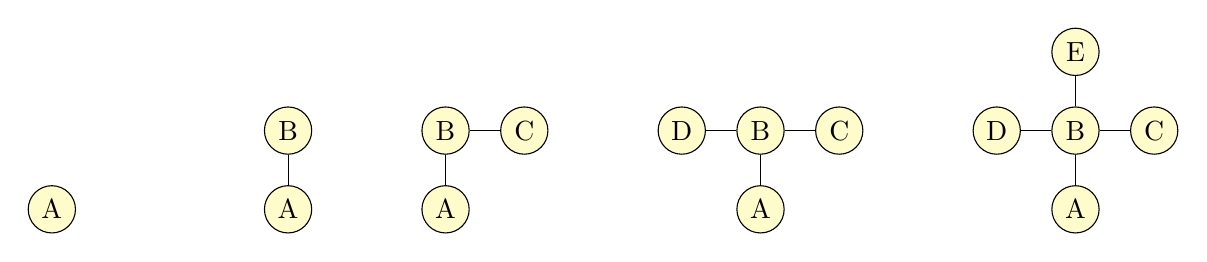
\begin{tikzpicture}[scale=1, every node/.style={circle, draw, fill=yellow!20, minimum size=6mm, inner sep=1pt}]

% n = 1
\node (A1) at (0,0) {A};

% n = 2
\node (A2) at (3,0) {A};
\node (B2) at (3,1) {B};
\draw (A2) -- (B2);

% n = 3
\node (A3) at (5,0) {A};
\node (B3) at (5,1) {B};
\node (C3) at (6,1) {C};
\draw (A3) -- (B3);
\draw (B3) -- (C3);

% n = 4
\node (A4) at (9,0) {A};
\node (B4) at (9,1) {B};
\node (C4) at (10,1) {C};
\node (D4) at (8,1) {D};
\draw (A4) -- (B4);
\draw (B4) -- (C4);
\draw (B4) -- (D4);

% n = 5
\node (A5) at (13,0) {A};
\node (B5) at (13,1) {B};
\node (C5) at (14,1) {C};
\node (D5) at (12,1) {D};
\node (E5) at (13,2) {E};
\draw (A5) -- (B5);
\draw (B5) -- (C5);
\draw (B5) -- (D5);
\draw (B5) -- (E5);

\end{tikzpicture}
\end{document}
